Consider, as an example, the graph $G_1$ in Figure \ref{treeboundpic}(a).  A spanning tree of $G_1$ is shown in Figure~\ref{treeboundpic}(b).  During the first iteration of the while-loop spanning Steps 3--6 of Algorithm~\ref{heuristic}, the four leaves (indicated as solid vertices) in Figure \ref{treeboundpic}(c) are inserted into the set $X$.  Thereupon the two end-clusters (highlighted in grey in the figure) are removed from the tree to obtain the smaller tree in Figure \ref{treeboundpic}(d).  The two leaves of this smaller tree are also inserted into $X$ after which the entire tree in the figure is pruned away (because the tree consists of a single end-cluster).  This process results in the secure dominating set $X=\{v_2,v_3,v_4,v_5,v_6,v_9\}$ of cardinality $6$ for the graph $G_1$.

\begin{figure}[htb]

\begin{center} \subfigure[]{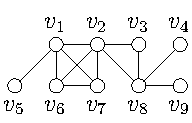
\includegraphics[height=1.6cm,bb=0 0 100 100]{examples/SecDomExa.pdf}} \hspace{0.5cm} \subfigure[]{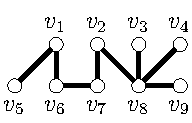
\includegraphics[height=1.6cm,bb=0 0 100 100]{examples/SecDomExa1.pdf}} \hspace{0.5cm} \subfigure[]{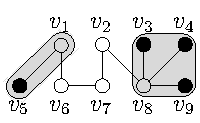
\includegraphics[height=1.6cm,bb=0 0 100 100]{examples/SecDomExb.pdf}} \hspace{0.5cm} \subfigure[]{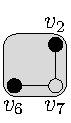
\includegraphics[height=1.6cm,bb=0 0 100 100]{examples/SecDomExc.pdf}} \end{center}

\vspace{-0.6cm}

\caption{(a) A graph $G_1$ for which $\gamma_s(G_1)=4$. (b) A spanning tree of $G_1$. (c)--(d) The result of identifying and pruning away end-clusters of the spanning tree in (b) according to Algorithm \ref{heuristic} to arrive at the secure dominating set $\{v_2,v_3,v_4,v_5,v_6,v_9\}$ of cardinality $6$ for $G_1$.} \label{treeboundpic} \end{figure}